\documentclass[aspectratio=169]{beamer}
\usetheme{Bruno}

\usepackage{comment}
\usepackage{graphicx}

\title[IoT for Rural Aqueducts using MBSE]{Towards a Modular IoT System Architecture for Rural Aqueducts using Model-Based Systems Engineering}
\author[Tecnológico de Costa Rica]{Anthony José Arguedas-Rodríguez \and María José Angulo-Campos \and Juan José Montero-Jiménez \and Juan José Rojas-Hernández}
\date{2025 IEEE International Symposium on Systems Engineering}

\begin{document}

\begin{frame}
    % Title in large font
    \begin{center}
        % Access the title variable
        {\LARGE \textbf{\inserttitle}} \\
        \vspace{0.5cm}
        {\insertauthor} \\
        \vspace{0.25cm}
        \includegraphics[height=2.3cm]{logo_delta.png} \includegraphics[height=1.3cm]{logo_tec.jpg} \\
        \vspace{0.25cm}
        {\insertdate}
    \end{center}
\end{frame}

\begin{comment}
# Initial slide

Greetings everyone and thank you for being here.
I am Anthony Arguedas, an undergraduate research assistant at Laboratorio Delta, at the Costa Rica Institute of Technology.
Today, I will be presenting our work titled "Towards a Modular IoT System Architecture for Rural Aqueducts using Model-Based Systems Engineering." 
\end{comment}

\begin{frame}
    \frametitle{Contents}
    \begin{itemize}
        \item IoT Systems in Rural Aqueducts Context
        \item ARCADIA Model-Based Systems Engineering (MBSE) Methodology
        \item Operational Need Analysis: What Rural Aqueducts Need to Accomplish
        \item System Need Analysis: What IoT Systems Must Accomplish for Rural Aqueducts
        \item Logical Architecture: A Generic and Modular IoT System
        \item Physical Architecture: A Case Study of ASADA Paso Ancho, Costa Rica
        \item Conclusions and Future Work
    \end{itemize}
\end{frame}

\begin{comment}
# Contents

In this presentation, we will start by presenting the context of IoT systems in rural aqueducts,
their capability gaps, and previous work done in the field of technology transfer from academia to rural aqueducts.

Then, we will introduce the ARCADIA Model-Based Systems Engineering Methodology, which we used to develop the system architecture that is the main contribution of our work.

We will through our design process across the four ARCADIA phases, culminating on a case study of a physical architecture
derived from our generic model for a particular rural aqueduct.
\end{comment}

\begin{frame}
    \frametitle{What are Rural Aqueducts?}

    \begin{columns}[T] % Align columns at the top
        \begin{column}{0.5\textwidth}
            \begin{enumerate}
                \item Self-managed
                \item Rural community-based
                \item Small-scale
                \item Limited staff
                \item Commonly resource-constrained
                \item Manual monitoring, inspection, and control methods
                \item Vulnerable to water loss and unreliable service
            \end{enumerate}
        \end{column}
        \begin{column}{0.5\textwidth}
            \begin{figure}
                \includegraphics[width=0.8\columnwidth]{images/asada.png}
                \caption{Aerial view of the water tank facility of ASADA Paso Ancho, Costa Rica.}
            \end{figure}
        \end{column}
    \end{columns}
\end{frame}

\begin{comment}
# What are Rural Aqueducts?

Firstly, we need to differentiate rural aqueducts from other water distribution networks by stating their main characteristics,
namely that they are self-managed, community-based, and commonly resource-constrained water resource administrators for rural areas.
Mentioning here that they are small-scale operations with limited staff is not redundant,
as larger operations are usually managed in a centralized manner.

They frequently rely on manual operational processes, and are vulnerable to water loss and unreliable service.

In the right we can see an aerial view of the water tank facility of ASADA Paso Ancho, a rural aqueduct in Costa Rica,
with which we are currently collaborating for the case study that will be presented at the end of this talk.
We can clearly see that these are small-scale operations without much infrastructure apart from the basic components
needed to store and distribute water using manual control.
\end{comment}

\begin{frame}
    \frametitle{\small IoT Systems in Rural Aqueducts Context}
    \framesubtitle{Previous Work on IoT Technology Transfer to Rural Aqueducts at Laboratorio Delta}

    \begin{columns}[T] % Align columns at the top
        \begin{column}{0.5\textwidth}
            \begin{figure}
                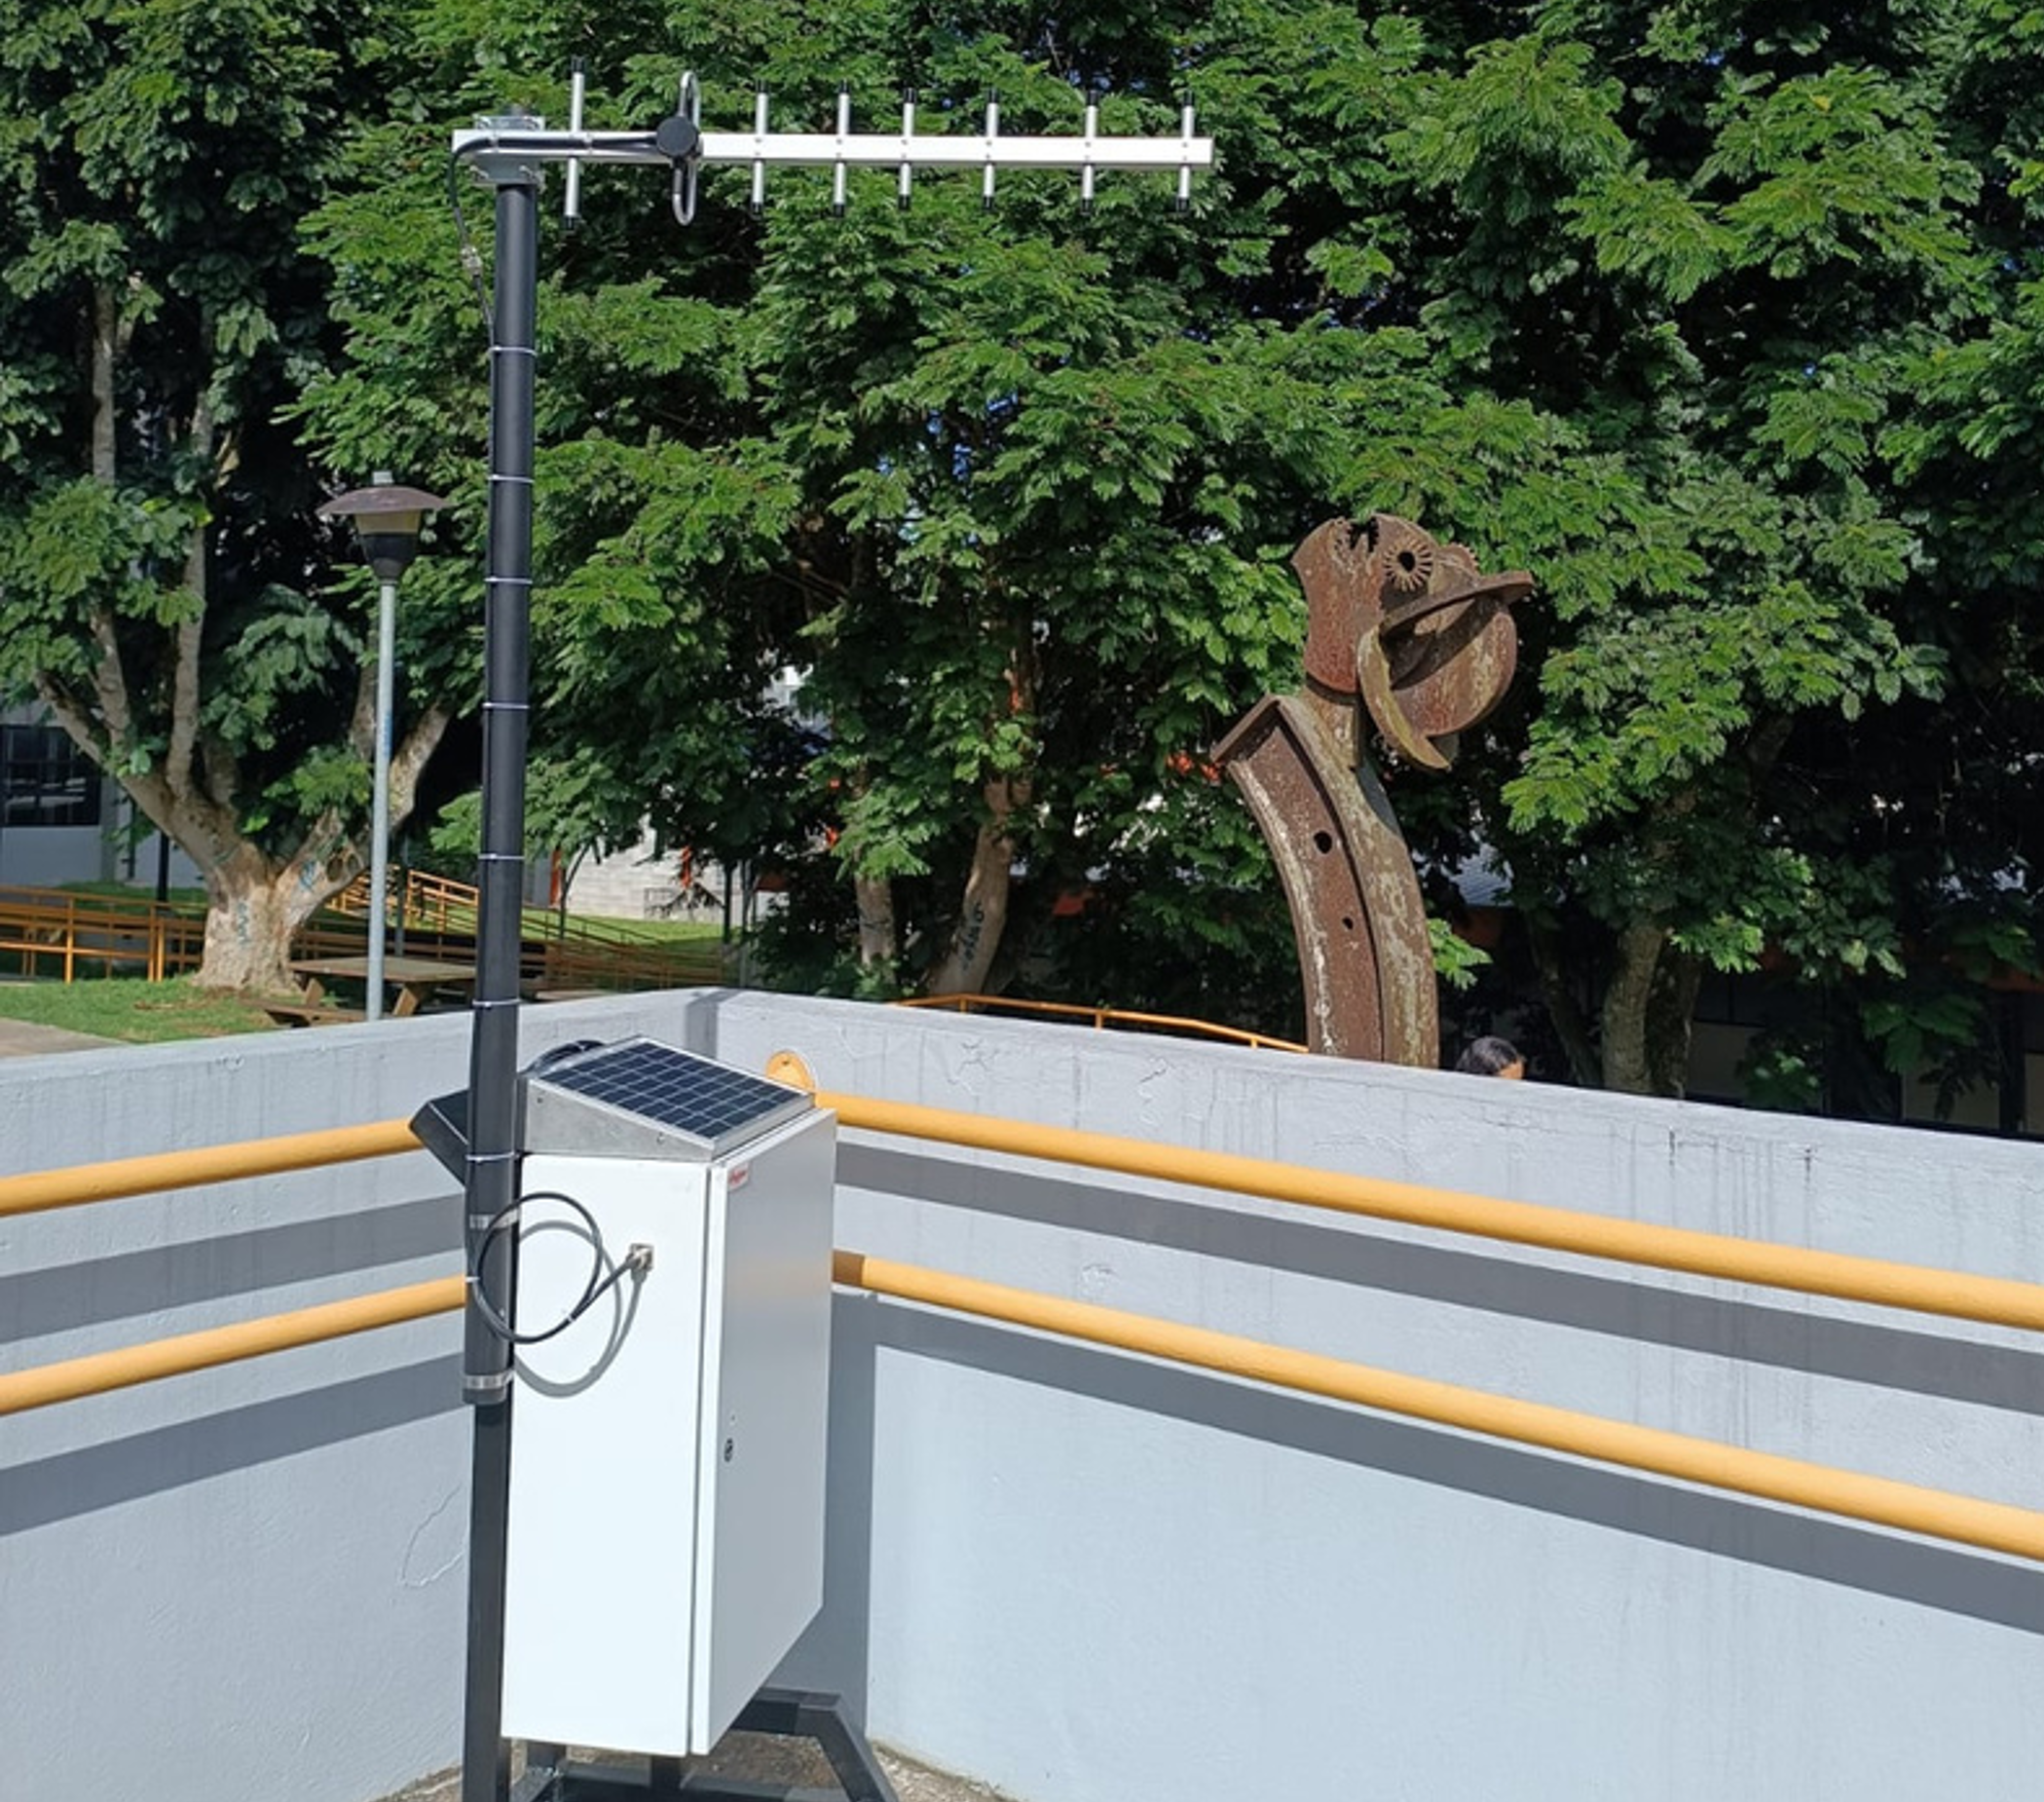
\includegraphics[width=0.7\columnwidth]{images/oviedo.png}
                \caption{IoT system developed by \cite{Oviedo2024} for ASADA Paso Ancho, Cartago.}
            \end{figure}
        \end{column}
        \begin{column}{0.5\textwidth}
            \begin{figure}
                \includegraphics[width=0.8\columnwidth]{images/solorzano.png}
                \caption{IoT system developed by \cite{Solorzano2021} for ASADA Playa Sámara, Nicoya.}
            \end{figure}
        \end{column}
    \end{columns}
\end{frame}

\begin{comment}
# Previous technology transfer work

An important inspiration for this work comes from previous efforts at Laboratorio Delta
to transfer IoT technology to rural aqueducts, such as two systems pictured here that were developed by previous lab members.

After the second project the need for standardization was identified,
because although the needs of desires that these systems addressed were similar,
the architectures were different, and in both cases the design process was started from almost from zero
although there was previous experience in the lab.
\end{comment}

\begin{frame}
    \frametitle{Research Questions}

    \begin{itemize}
        \item \textbf{RQ1:} Are there existing systems engineering-based (including ARCADIA MBSE) architectures for the design of IoT systems for rural aqueducts?
        \item \textbf{RQ2:} If they exist, are the architectures generic and modular?
        \item \textbf{RQ3:} What are the needs and desires of rural aqueducts that can be addressed by IoT systems?
        \item \textbf{Contribution:} A generic system architecture for rural aqueducts, developed using the ARCADIA method
    \end{itemize} 
\end{frame}

\begin{comment}
The identified capability gaps and the potential for standardization in the design of IoT systems for rural aqueducts
led us to formulate the these research questions.

We aimed to surface existing architectures that were developed using systems engineering-based methodologies, and to
assess if they were generic and modular so as to allow for adaptation to different contexts.

Importantly, we found no previous works that applied the ARCADIA MBSE method, or any systematic approach altogether
to this problem domain, despite there being a wealth of literature on IoT systems for rural aqueducts.

Thus, we decided to contribute a generic system architecture for rural aqueducts,
developed using the ARCADIA method, for which the very stage was to identify the needs and desires of rural aqueducts that can be addressed by IoT systems, as exemplified by research question 3.
\end{comment}

\begin{frame}
    \frametitle{The ARCADIA MBSE Methodology}

    \begin{figure}
        \centering
        \includegraphics[width=0.9\textwidth]{images/phases_arcadia.png}
        \caption{Phases of the ARCADIA Model-Based Systems Engineering Methodology and its associated Language and Tool Capella.}
    \end{figure}
\end{frame}

\begin{comment}
# The ARCADIA MBSE Methodology

Our work finds its basis in a systems engineering approach that employs an exhaustive and rigorous abstraction
of the system to be designed, which we know of as a model.
\end{comment}

\begin{frame}
    \frametitle{\small Operational Need Analysis}
    \framesubtitle{Extracting Generic Needs and Desires about IoT Systems in Rural Aqueducts using NLP}

    \begin{table}
        \centering
        \caption{Needs and desires extracted from paper full text embeddings using BERTopic.}
        \begin{tabular}{c p{6cm}}
            Code & Need or desire \\
            \hline
            ND1.1 & Identify sources of water pollution \\ %
            ND1.2 & Monitor water pollution \\ %
            ND2 & Monitor water pH \\ %
            ... & ... \\ %
            ND52 & MQTT node communication \\
            ND53 & Mobile network connectivity \\
            ND54 & WiFi connectivity \\
            ND55 & LoRaWAN connectivity \\
            \hline
        \end{tabular}
        \label{tab:clusters}
    \end{table}
\end{frame}

\begin{frame}
    \frametitle{\small Operational Need Analysis: Operational Capabilities}
    \framesubtitle{1: Provide high-quality water, 2: Comply with water quality standards and 4: Share data with external entities}

    \begin{figure}
        \centering
        
\includegraphics[width=\textwidth]{images/opcap1.jpg}
        \caption{Operational Need Analysis for rural aqueducts, reduced to the activities involved in Capabilities 1, 2 and 4.}
    \end{figure}
\end{frame}

\begin{frame}
    \frametitle{\small Operational Need Analysis}
    \framesubtitle{Operational Capability 3: Mitigate water loss}

    \begin{figure}
        \centering
        \includegraphics[width=0.9\textwidth]{images/opcap3.jpg}
        \caption{Operational Need Analysis for rural aqueducts, reduced to the activities involved in Capability 3.}
    \end{figure}
\end{frame}

\begin{frame}
    \frametitle{\small System Need Analysis: System Capabilities}
    \framesubtitle{1: Provide water quality data, 5: Share data with external entities}

    \begin{figure}
        \centering
        
\includegraphics[width=0.9\textwidth]{images/scap1-5.jpg}
        \caption{System Need Analysis for IoT systems in rural aqueducts, reduced to the activities involved in Capabilities 1 and 5.}
    \end{figure}
\end{frame}

\begin{frame}
    \frametitle{\small System Need Analysis: System Capabilities}
    \framesubtitle{2: Provide water loss data, 3: Provide water supply and demand data, 4: Control water distribution}

    \begin{figure}
        \centering
        
\includegraphics[width=0.85\textwidth]{images/scap2-3-4.jpg}
        \caption{System Need Analysis for IoT systems in rural aqueducts, reduced to the activities involved in Capabilities 2, 3 and 4.}
    \end{figure}
\end{frame}

\begin{frame}
    \frametitle{\small Logical Architecture Definition}
    \framesubtitle{Implementing modularity with end-user and environmental interactions}

    \begin{figure}
        \centering
        
\includegraphics[width=0.77\textwidth]{images/separation.jpg}
        \caption{Logical architecture for IoT systems in rural aqueducts, reduced to the logical componentes that interact with end-users and the environment.}
    \end{figure}
\end{frame}

\begin{frame}
    \frametitle{\small Logical Architecture Definition}
    \framesubtitle{Implementing modularity with buses, queues, and pub/sub channels}

    \begin{figure}
        \centering
        
\includegraphics[width=0.75\textwidth]{images/component_exchanges.jpg}
        \caption{Logical architecture for IoT systems in rural aqueducts, reduced to logical components and their component exchanges.}
    \end{figure}
\end{frame}

\begin{frame}
    \frametitle{\small Physical Architecture Definition}
    \framesubtitle{Implementing Logical Components}

    \begin{figure}
        \centering
        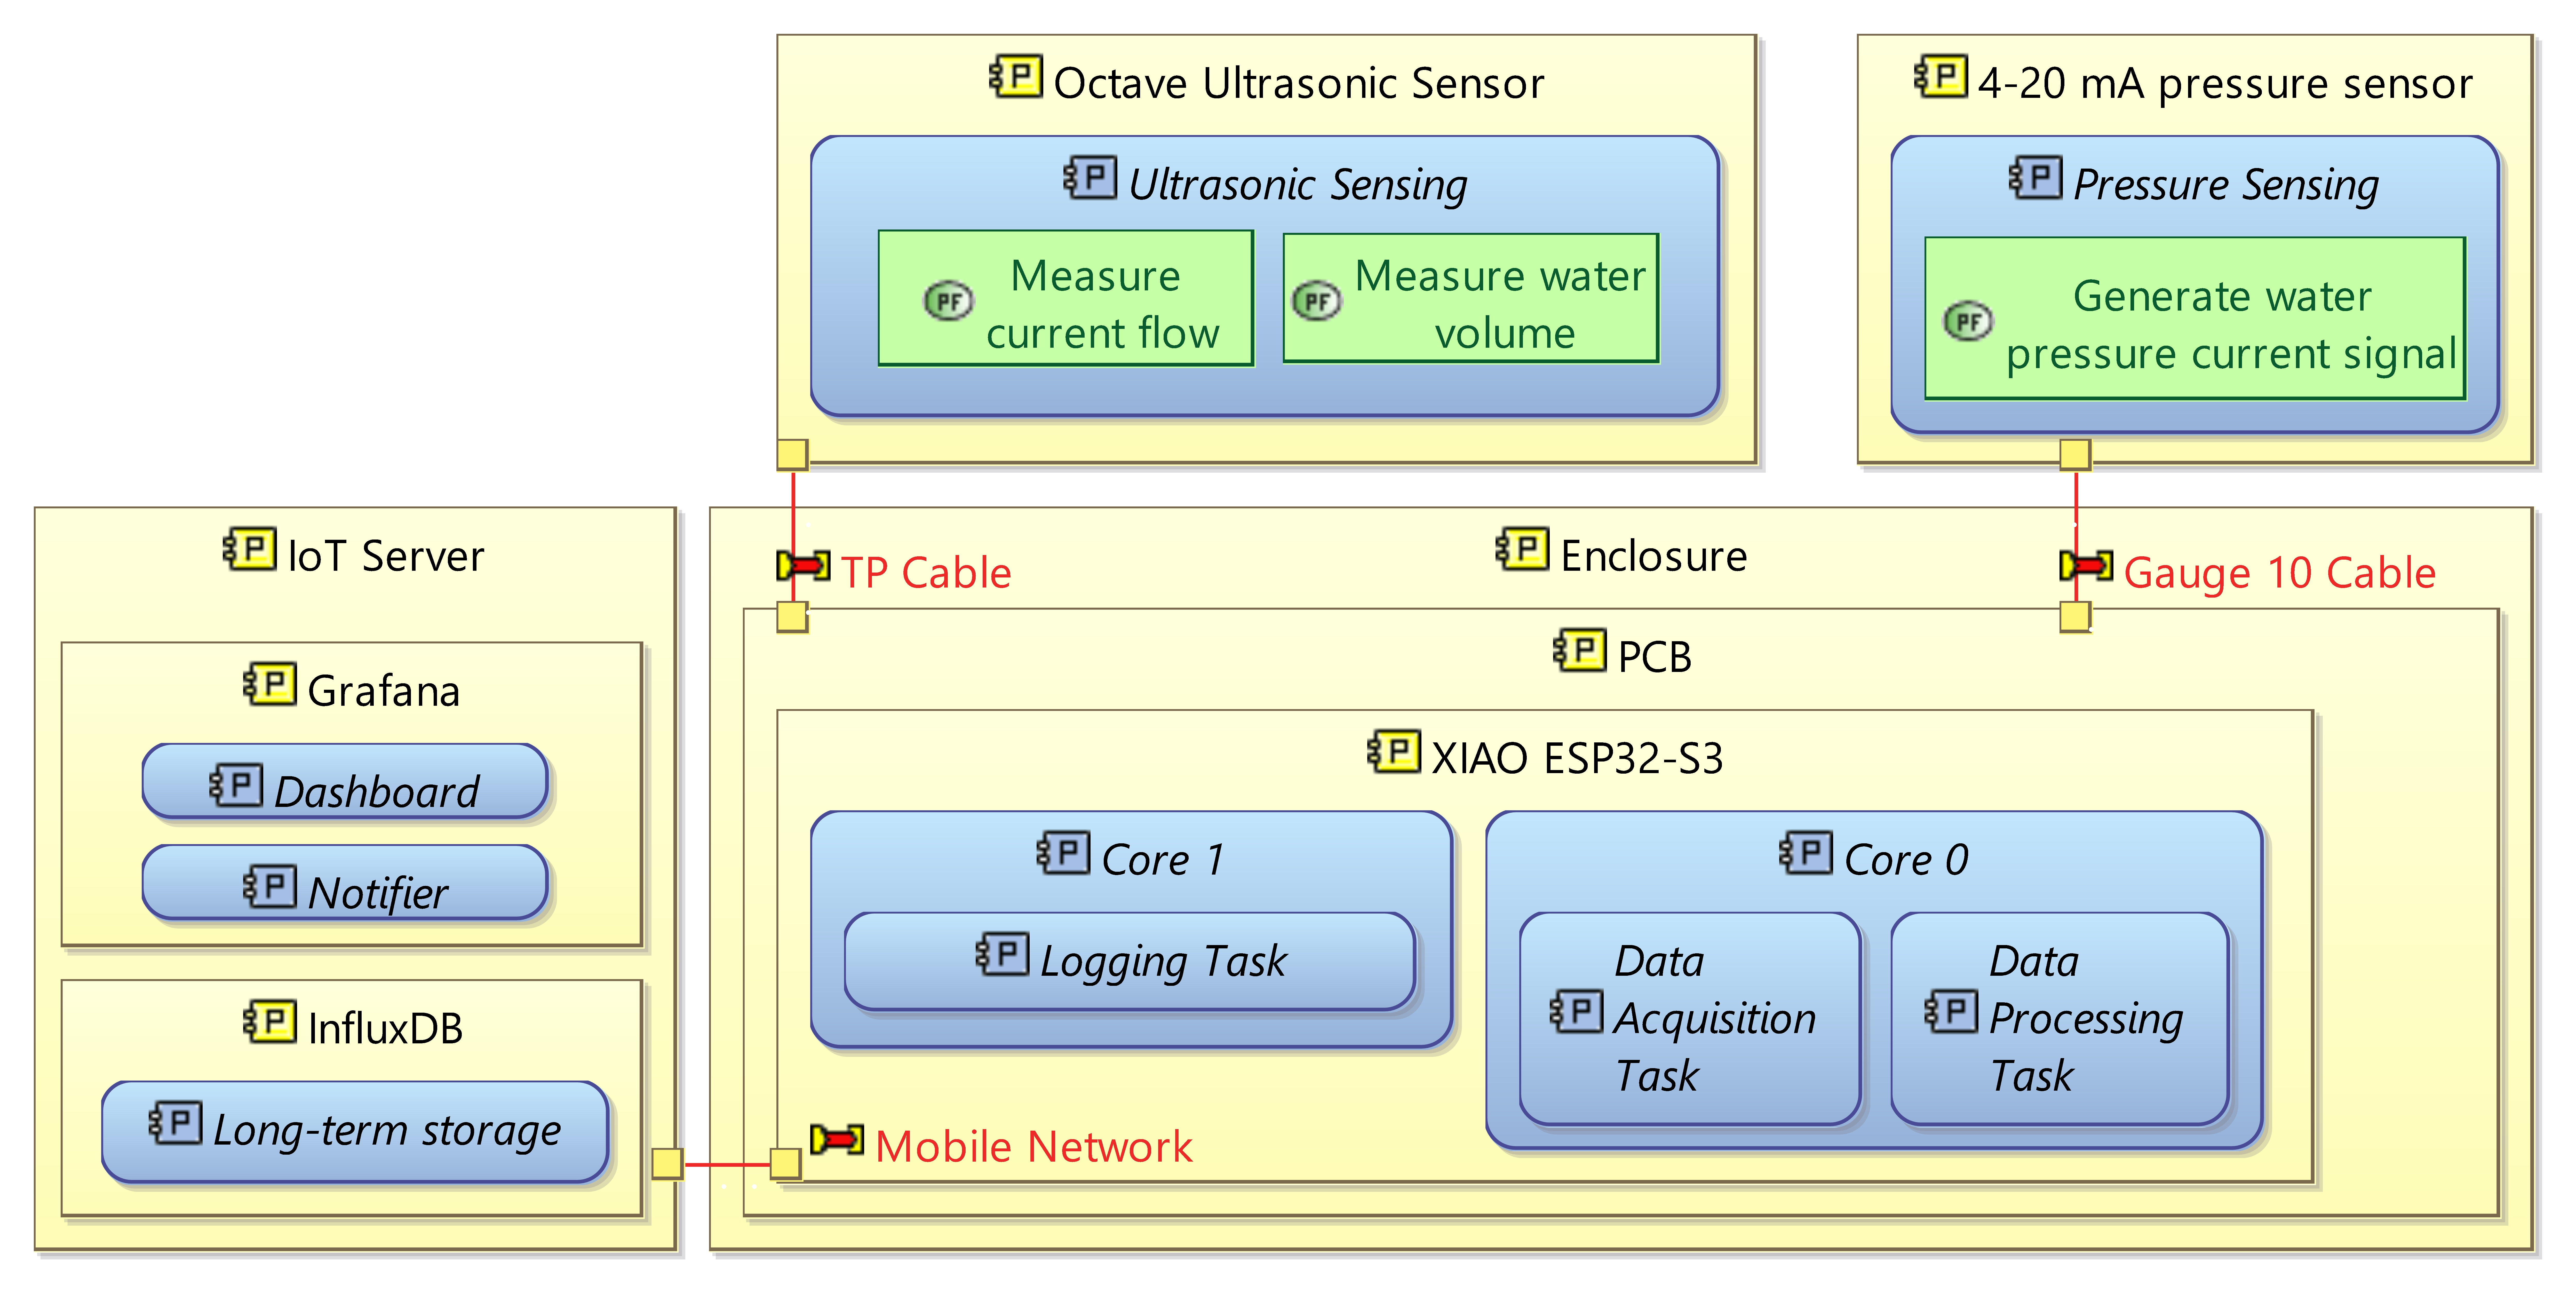
\includegraphics[width=0.65\textwidth]{images/physical_implementation.jpg}
        \caption{Physical architecture for IoT systems in rural aqueducts, reduced to the Physical Components implementing the Logical Architecture.}
    \end{figure}
\end{frame}

\begin{frame}
    \frametitle{\small Physical Architecture Definition}
    \framesubtitle{Introducing Implementation-Specific Functions}

    \begin{figure}
        \centering
        
\includegraphics[width=0.9\textwidth]{images/physical_new.jpg}
        \caption{Physical architecture for IoT systems in rural aqueducts, reduced to implementation-specific functions not found in the Logical Architecture.}
    \end{figure}
\end{frame}

\begin{frame}
    \frametitle{Conclusions and Future Work}

    \begin{itemize}
        \item Generality was introduced by extracting needs and desires from a wide range of literature using data mining techniques.
        \item The application of the ARCADIA MBSE method enabled traceability from needs to logical and even physical architecture, and technology-agnostic design.
        \item Modularity was achieved by separating end-user and environmental interactions, and by using buses, queues, and pub/sub channels for component exchanges.
        \item The presented architecture can be adapted to a practical implementation, for example by technology transfer initiatives.
        \item Future work should strengthen the data mining pipeline by including more sources of information, and further developing the physical architecture with more case studies.
    \end{itemize}
\end{frame}

\begin{frame}[allowframebreaks]
    \frametitle{References}
    \bibliographystyle{IEEEtran}
    \bibliography{refs}
\end{frame}

\begin{frame}
    \frametitle{\small Backup Slide}
    \framesubtitle{NLP Pipeline for Generic Needs and Desires Extraction}

    \begin{figure}
        \centering
        \includegraphics[width=\textwidth]{images/bertopic.png}
        \caption{Process of extracting generic needs and desires about IoT systems in rural aqueducts from published literature.}
    \end{figure}
\end{frame}

\end{document}